\section{PWM opsætning}

Testen bruges til at fastslå hvorvidt det PWM signal, der genereres af main controller, udsendes med korrekt frekvens og pulsbredde. Testen foregår ved at ændre værdien af compare-registeret\footnote{Se implementation view i \textit{Systemarkitektur og Design}} . Ændringer i compare registerets værdi bør medføre ændringer af pulsbredde i det PWM signal der udsendes fra main controller. 

Indledningsvis indstilles compare-registeret med værdi på 16000, derefter ændres værdien til 24000 og til sidst sættes compare-registerets værdi til 32000. Ved brug af oscilloskop kontrolleres om PWM signal har den korrekte pulsbredde. 

Nedenfor ses en tabel der viser hvordan testen forløb. Efter tabellen vises oscilloskop billeder taget under testen. 

\vspace{0.50cm}

\begin{table}[H]
	\centering
		\begin{tabular}{|c|c|c|c|}
			\hline
			Værdi compare reg. & Frekvens & Forventet pulsbredde & Faktisk pulsbredde \\ \hline
			16000 & 245 Hz & 1.00 ms & 1.00 ms \\ \hline			
			24000 & 245 Hz & 1.50 ms & 1.50 ms \\ \hline
			32000 & 245 Hz & 2.00 ms & 2.00 ms \\ \hline
		\end{tabular}
	\caption{Test resultat}
\end{table}

\vspace{0.50cm}

Figur \ref{fig:PWM_1} vises PWM signal hvor compare register har værdi på 16000. 

\begin{figure}[H]
\centering
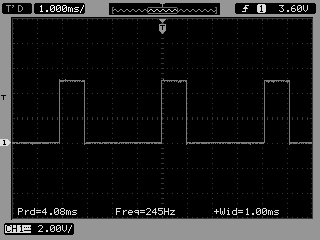
\includegraphics[width=0.7\textwidth]{Billeder/Test/PWM_16000.png}
\vspace{-0.0cm}
\caption{PWM signal - Compare register 16000}
\label{fig:PWM_1}
\end{figure}

\newpage

Figur \ref{fig:PWM_2} vises PWM signal hvor compare register har værdi på 24000. 
\begin{figure}[H]
\centering
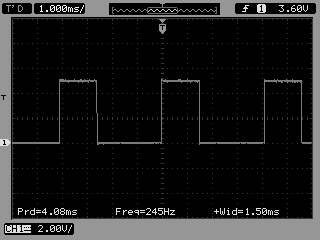
\includegraphics[width=0.7\textwidth]{Billeder/Test/PWM_24000.png}

\caption{PWM signal - Compare register 24000}
\label{fig:PWM_2}
\end{figure}

\vspace{0.5cm}

Figur \ref{fig:PWM_3} vises PWM signal hvor compare register har værdi på 32000. 
\begin{figure}[H]
\centering
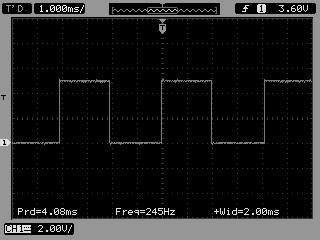
\includegraphics[width=0.7\textwidth]{Billeder/Test/PWM_32000.png}
\vspace{-0.0cm}
\caption{PWM signal - Compare register 32000}
\label{fig:PWM_3}
\end{figure}